\chapter{Materials and Methods} \label{sec:mm}

This chapter covers the images that were available for analysis, how they were processed, and which methods were applied to analyse them. Detailed results of the implementation of these methods are then presented and discussed in Section \ref{sec:implementation}.

\section{Immune cells dataset}

\subsection{Setup}

The images that were used for the purpose of this research were provided by the Laboratory of Immune Cell Visualisation and Examination (LIVE) at the Institute of Infection, Immunity \& Inflammation at the University of Glasgow. The images were captured from 384-well plates with a commercial INCell Analyzer 2000. As established in Section \ref{bg:immunesystem}, the type of immune cells we are studying are T-cells and dendritic cells (DCs). Each plate to be imaged in the INCell Analyzer contains a grid of wells. Each of those wells is assigned a label and an experimental condition. T-cells, dendritic cells, and compounds related to the experimental conditions are injected in the well. In order to be able to distinguish between them, cells are loaded with fluorescent dyes: the T-cells are dyed with a green dye (CSFE dye), and the dendritic cells are dyed with a red dye (CMTPX dye). After imaging, we obtain three field-of-view images per well:

[should I add an image of a plate of wells for illustration if that is not clear to a casual reader?]

\begin{itemize}
    \item a Brightfield image, which shows both T-cells and dendritic cells (Figure \ref{fig:fov_brightfield})
    \item an image showing only the T-cells, which has been captured thanks to the fluorescent green dye (Figure \ref{fig:fov_fitc})
    \item an image showing only the dendritic cells, which has been captured thanks to the fluorescent red dye (Figure \ref{fig:fov_tr}).
\end{itemize}

\begin{figure}[h]!
    \centering
    \begin{subfigure}[h!]{0.3\textwidth}
        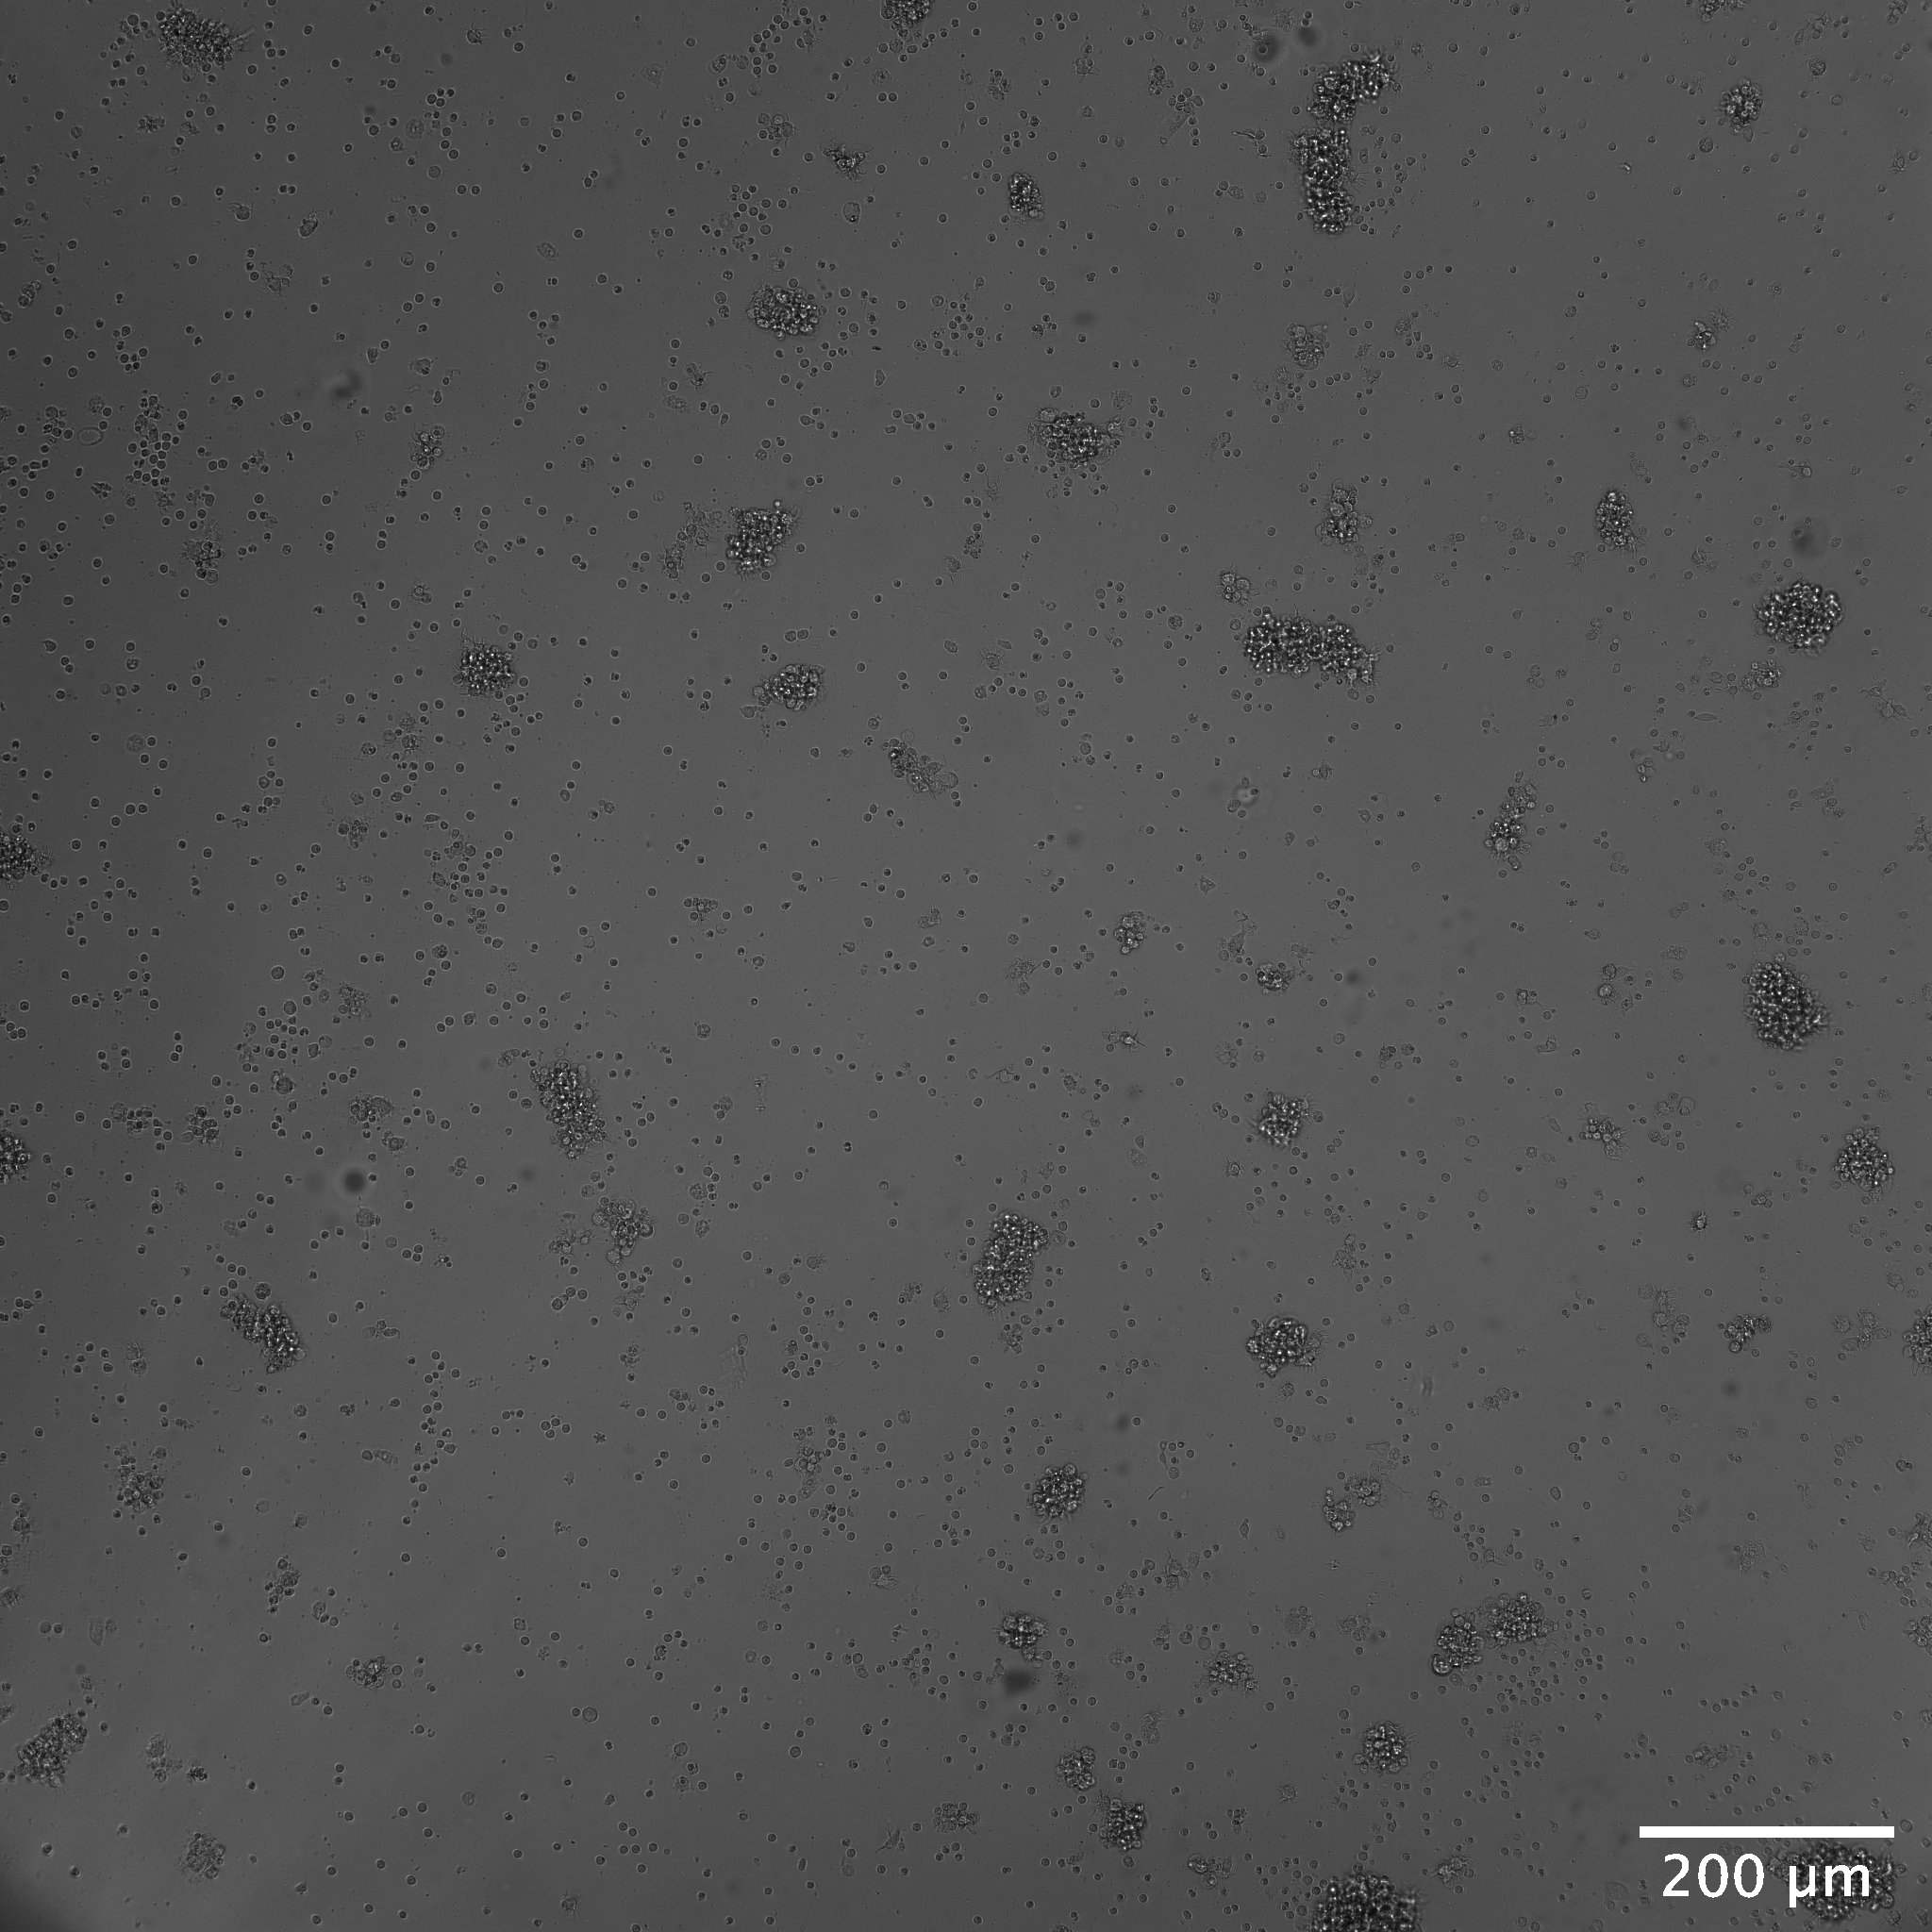
\includegraphics[width=\textwidth]{dissertation/figures/example_Brightfield_L20.jpg}
        \caption{Brightfield view}
        \label{fig:fov_brightfield}
    \end{subfigure}
    \begin{subfigure}[h!]{0.3\textwidth}
        
\includegraphics[width=\textwidth]{dissertation/figures/example_FITC_L20.png}
        \caption{Green dye (T-cells) view}
        \label{fig:fov_fitc}
    \end{subfigure}
    \begin{subfigure}[h!]{0.3\textwidth}
        \includegraphics[width=\textwidth]{dissertation/figures/example_TexasRed_L20.png}
        \caption{Red dye (DCs) view}
        \label{fig:fov_tr}
    \end{subfigure}
    \caption{Microscope images extracted from the dataset showing each view obtained with the capture system. Brightness has been adjusted for \subref{fig:fov_fitc}, \subref{fig:fov_tr} for details to come through.}
    \label{fig:fov}
\end{figure}

\subsection{Experimental conditions}

8,000 dendritic cells and 8,000 T-cells were cultured in each of the 384 wells. The INCell Analyzer 2000 captured an image of around 25\% of each well. The dendritic cells were cultured from bone marrow cells obtained from mice. T-cells were obtained from mice's lymphoid tissues. 70 to 90\% of the T-cells in these mice's immune system expressed a receptor for the antigen Ovalbumin (OVA) peptide, which means they recognised it well.

Each well in a plate was associated with an experimental condition:
\begin{itemize}
    \item The well are injected with one of 45 drug compounds, % aimed at inhibiting the strength of bonds between immune cells
    \item These compounds could be injected at a bigger or lesser concentration,
    \item Moreover, one of two types of antigens could be injected to further stimulate the cells.
\end{itemize}

We are interested in using the latter as a label for our images, as it gives us a smaller number of categories to look at. More specifically, there are three categories of stimulation:
\begin{itemize}
    \item No stimulation
    \item Stimulation with Ovalbumin (OVA) peptide, which is the antigen that should be recognised by most T-cells in the well
    \item Stimulation with Concanavalin A (ConA), an antigen which cross-links T-cells receptors with a molecule on DCs that would hold the OVA peptide antigen and show it to T-cells
\end{itemize}

\subsection{Selecting images} \label{subsec:selecting_dataset}

There was a large amount of images available from different well plates with the different experimental conditions described above. However, each set of images corresponding to a plate represented about 8 GB of data on average. Moving images through disks or cloud filing system thus represented substantial time and was vulnerable to transfer errors. Hence, a limited number of plates were selected for training and evaluation to make sure their consistency could be validated. Chosen plates were selected to best represent the experimental conditions we have chosen to study.

\begin{itemize}
    \item \textbf{The `full' dataset}: this dataset contains an equal number of images in the three categories of stimulation: no stimulation, stimulation with OVA, and simulation with ConA. This is to fight issues of class imbalance when training the model.
    \item \textbf{The simpler `dual' dataset}, with two categories: this dataset contains an equal number of images in two categories: no stimulation, and stimulation with OVA peptide. This was selected under the hypothesis that if useful results cannot be obtained with a dataset containing images from all categories, a deep learning model might be able to perform better with two.
    \item \textbf{The `DMSO' dataset}: Dimethyl sulfoxide (DMSO) is a solvent that helps solubilise the investigated drug compounds, as most compounds are not initially water soluble. When in solution, drug compounds should be more bioavailable and have more of a biological impact. DMSO images in the dataset only include DMSO and no drugs, and act as a control. However, this should show the most difference in between stimulation categories as they do not show the impact of drugs.
\end{itemize}

These datasets are summarised in Table \ref{table:datasets}.

\begin{table}[h]
\centering
\caption{Number of images in each category of stimulation by dataset. Both full and dual datasets should have no issues with class imbalance.}
\begin{tabular}{|l|r|r|r|}
\rowcolor[HTML]{EFEFEF}
\hline
Dataset & Unstimulated & OVA & ConA \\ \hline
Full    & 9,800        & 9,800 & 9,800    \\
Dual    & 6,900        & 6,900 & 0    \\
DMSO    & 4,600        & 2,600   & 2,600   \\ \hline
\end{tabular}
\label{table:datasets}
\end{table}

\subsection{Pre-processing} \label{subsec:preproc}
The datasets obtained from this setup consisted of 2048x2048 16-bit images in TIFF format, captured by a 12-bit camera. As mentioned above, each ``image” consists in fact of a set of three views: the green fluorescent image (T-cells), the red fluorescent image (dendritic cells), and the brightfield image. The brightfield images show both cell types and can be used for diagnostic purposes when deciding on pre-processing methods, but were otherwise discarded and not used for further analysis.

Each of the images sized about 8MB, and represented 4,194,304 pixels. This represented an issue of very high dimensions to handle for a model. Each plate also had about 400 wells, which corresponds to 800 images when counting both the T-cells image and the DCs image. This meant that we had quite a limited amount of images to feed into any kind of model.

Moreover, Figures \ref{fig:fov_fitc} and \ref{fig:fov_tr} show that even to the naked eye, the smaller white dots could easily be confused for dust on the screen, and could be as confusing for a deep learning model trying to learn features from an image as they are for us. Furthermore, images remained of very high dimensions. Indeed, a basic autoencoder with three 2x2 downsampling operations would yield around 500,000 pixel points from a 2048x2048 input image, which is a very high number for a visualisation technique like t-SNE or UMAP.

\bigskip
\subsubsection{Sliding window}

\hfill\\
\hfill\\
To resolve this issue, the first idea was to make the images more manageable by a neural network by cropping a set square subsection of the image of smaller dimensions, for example a square of 250x250 pixels. However, this would leave the issue of having only limited input to train a neural network. Instead, images were pre-processed by passing a sliding window over the image, creating patches of images per file. This quickly expanded the size of the dataset, making it as large as 58,000 samples in some cases. Smaller images also made more sense to the naked eye, hence the assumption was made that a trained neural network would perform better on this gridded dataset than on a full-image dataset.

\bigskip
\subsubsection{Normalisation}

\hfill\\
\hfill\\
Each sub-image was normalised with min-max normalisation (\autoref{equation:minmax}) to get a [0, 1] range of pixel values. It is common to normalise imaging data to the floating-point [0, 1] range over keeping an integer representation of an image, as integers are subject to saturation and rounding error. We are using min-max normalisation as not all images in our dataset have 0 as their minimum value.

\begin{equation}
    minmax(x) = \frac{x - min(x)}{max(x) - min(x)}
\label{equation:minmax}
\end{equation}

\bigskip
\subsubsection{Noise and outlier detection}

\hfill\\
\hfill\\
From analysing the images, it was also found that some images contained many pixels in the range of [0, 255] before normalisation. Moreover, such pixels usually seemed to correspond to background noise as shown in Figure \ref{fig:bgnoise}. The fact that these lie in the range of an 8-bit image pixel range might be coincidental, or the result of the way the imaging system captured non-dyed elements in the well. The immunology researcher providing the images confirmed that this noise was present in some images read from specific plates. Wells in early experiments were injected with additional cells as researchers thought this made the cells behave more naturally, however this was later found to have no real impact. These cells were not dyed, but some of their details still came through the imaging system. Although this background was not always visible to the naked eye, we did not want those pixel values to confuse a neural network model. Hence, values below 255 in images were clipped to 255 before min-max normalisation was applied.

\begin{figure}[h!]
    \centering
    \begin{subfigure}[h!]{0.99\textwidth}
        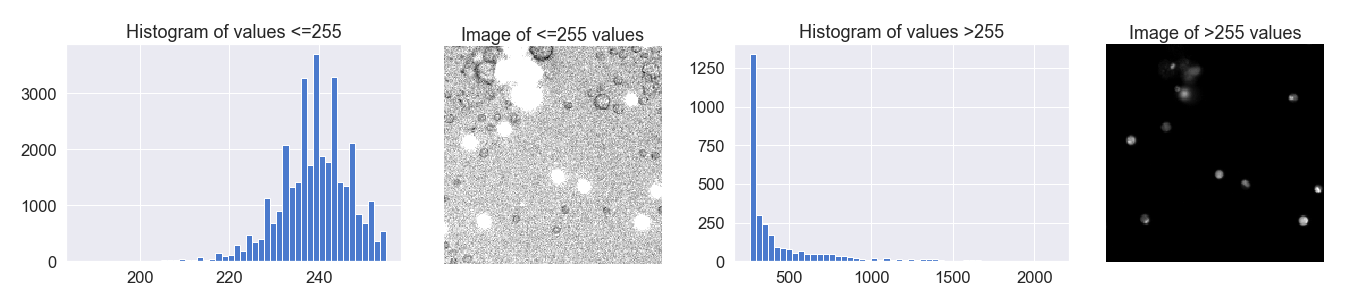
\includegraphics[width=\textwidth]{dissertation/figures/background_noise_true.png}
        \caption{Histogram and image analysis for a sub-image with noisy cells in the background}
        \label{fig:bgnoisetrue}
    \end{subfigure}

    \begin{subfigure}[h!]{0.99\textwidth}
        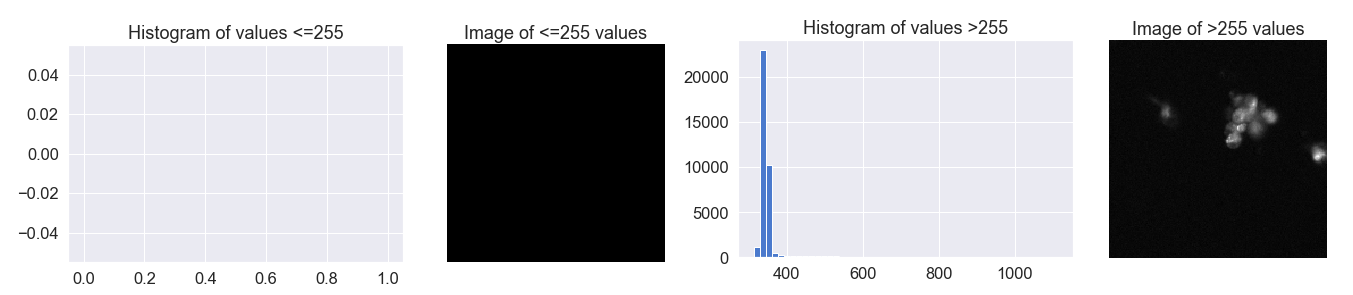
\includegraphics[width=\textwidth]{dissertation/figures/background_noise_false.png}
        \caption{Histogram and image analysis for a sub-image with no noisy cells in the background}
        \label{fig:bgnoisefalse}
    \end{subfigure}

    \caption{Histogram and image analysis for background noise detection}
    \label{fig:bgnoise}

\end{figure}

As described above, the provided images sometimes contained some background noise. Furthermore, some images contained larger amounts of noise coming from defects in the wells, such as water droplets. This is illustrated in Figure \ref{fig:noisyimage}. Their pixel value distribution followed the [0, 255] range as described above, but these values also covered the whole sub-image and no cells of interest were present in those patches. Removing them entirely from the dataset would make it more difficult to reason about whole images. Indeed, by pre-processing full images with a sliding window, each full image is represented by a patch of a set number of sub-images. This would then create inconsistencies in the amount of sub-images per image file. Instead of removing them, it was decided to keep them in to see if a neural network could make sense of them as a category. Noisy sub-images were labelled as ``Faulty".

\begin{figure}[h!]
    \centering
    \begin{subfigure}[h!]{0.3\textwidth}
        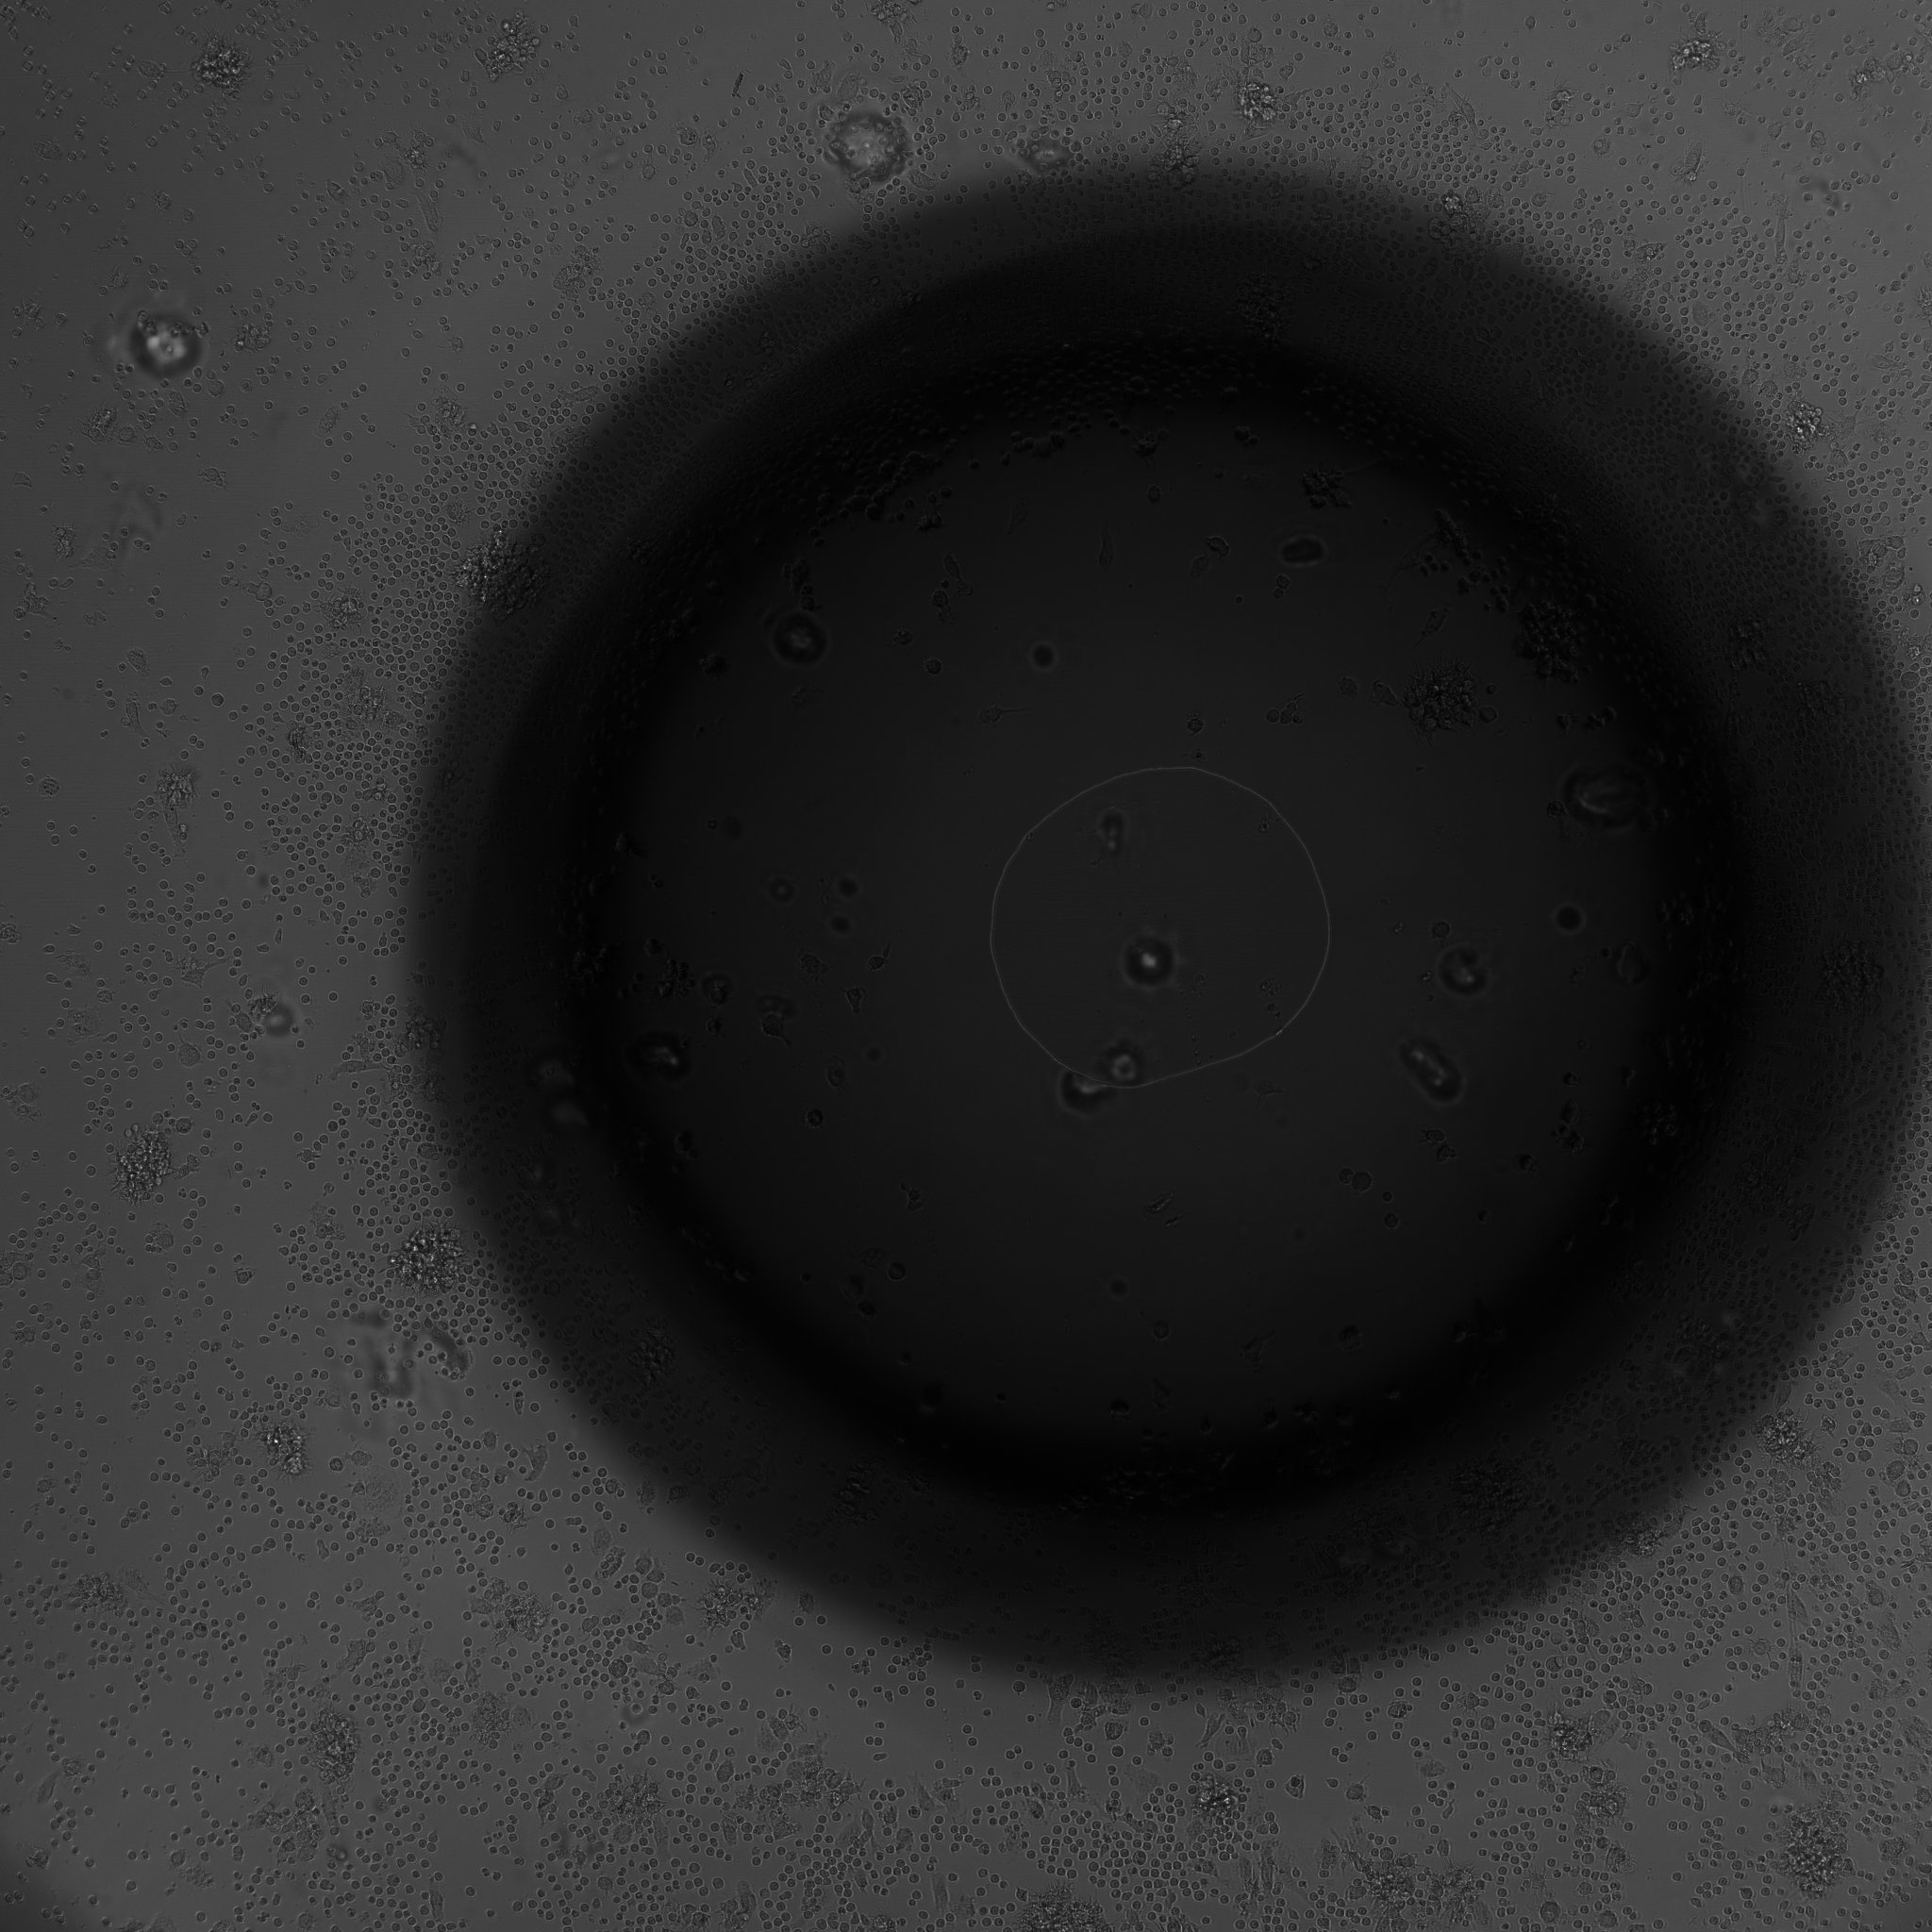
\includegraphics[width=\textwidth]{dissertation/figures/faulty_brightfield.jpg}
        \caption{Brightfield view}
    \end{subfigure}
    \begin{subfigure}[h!]{0.3\textwidth}
        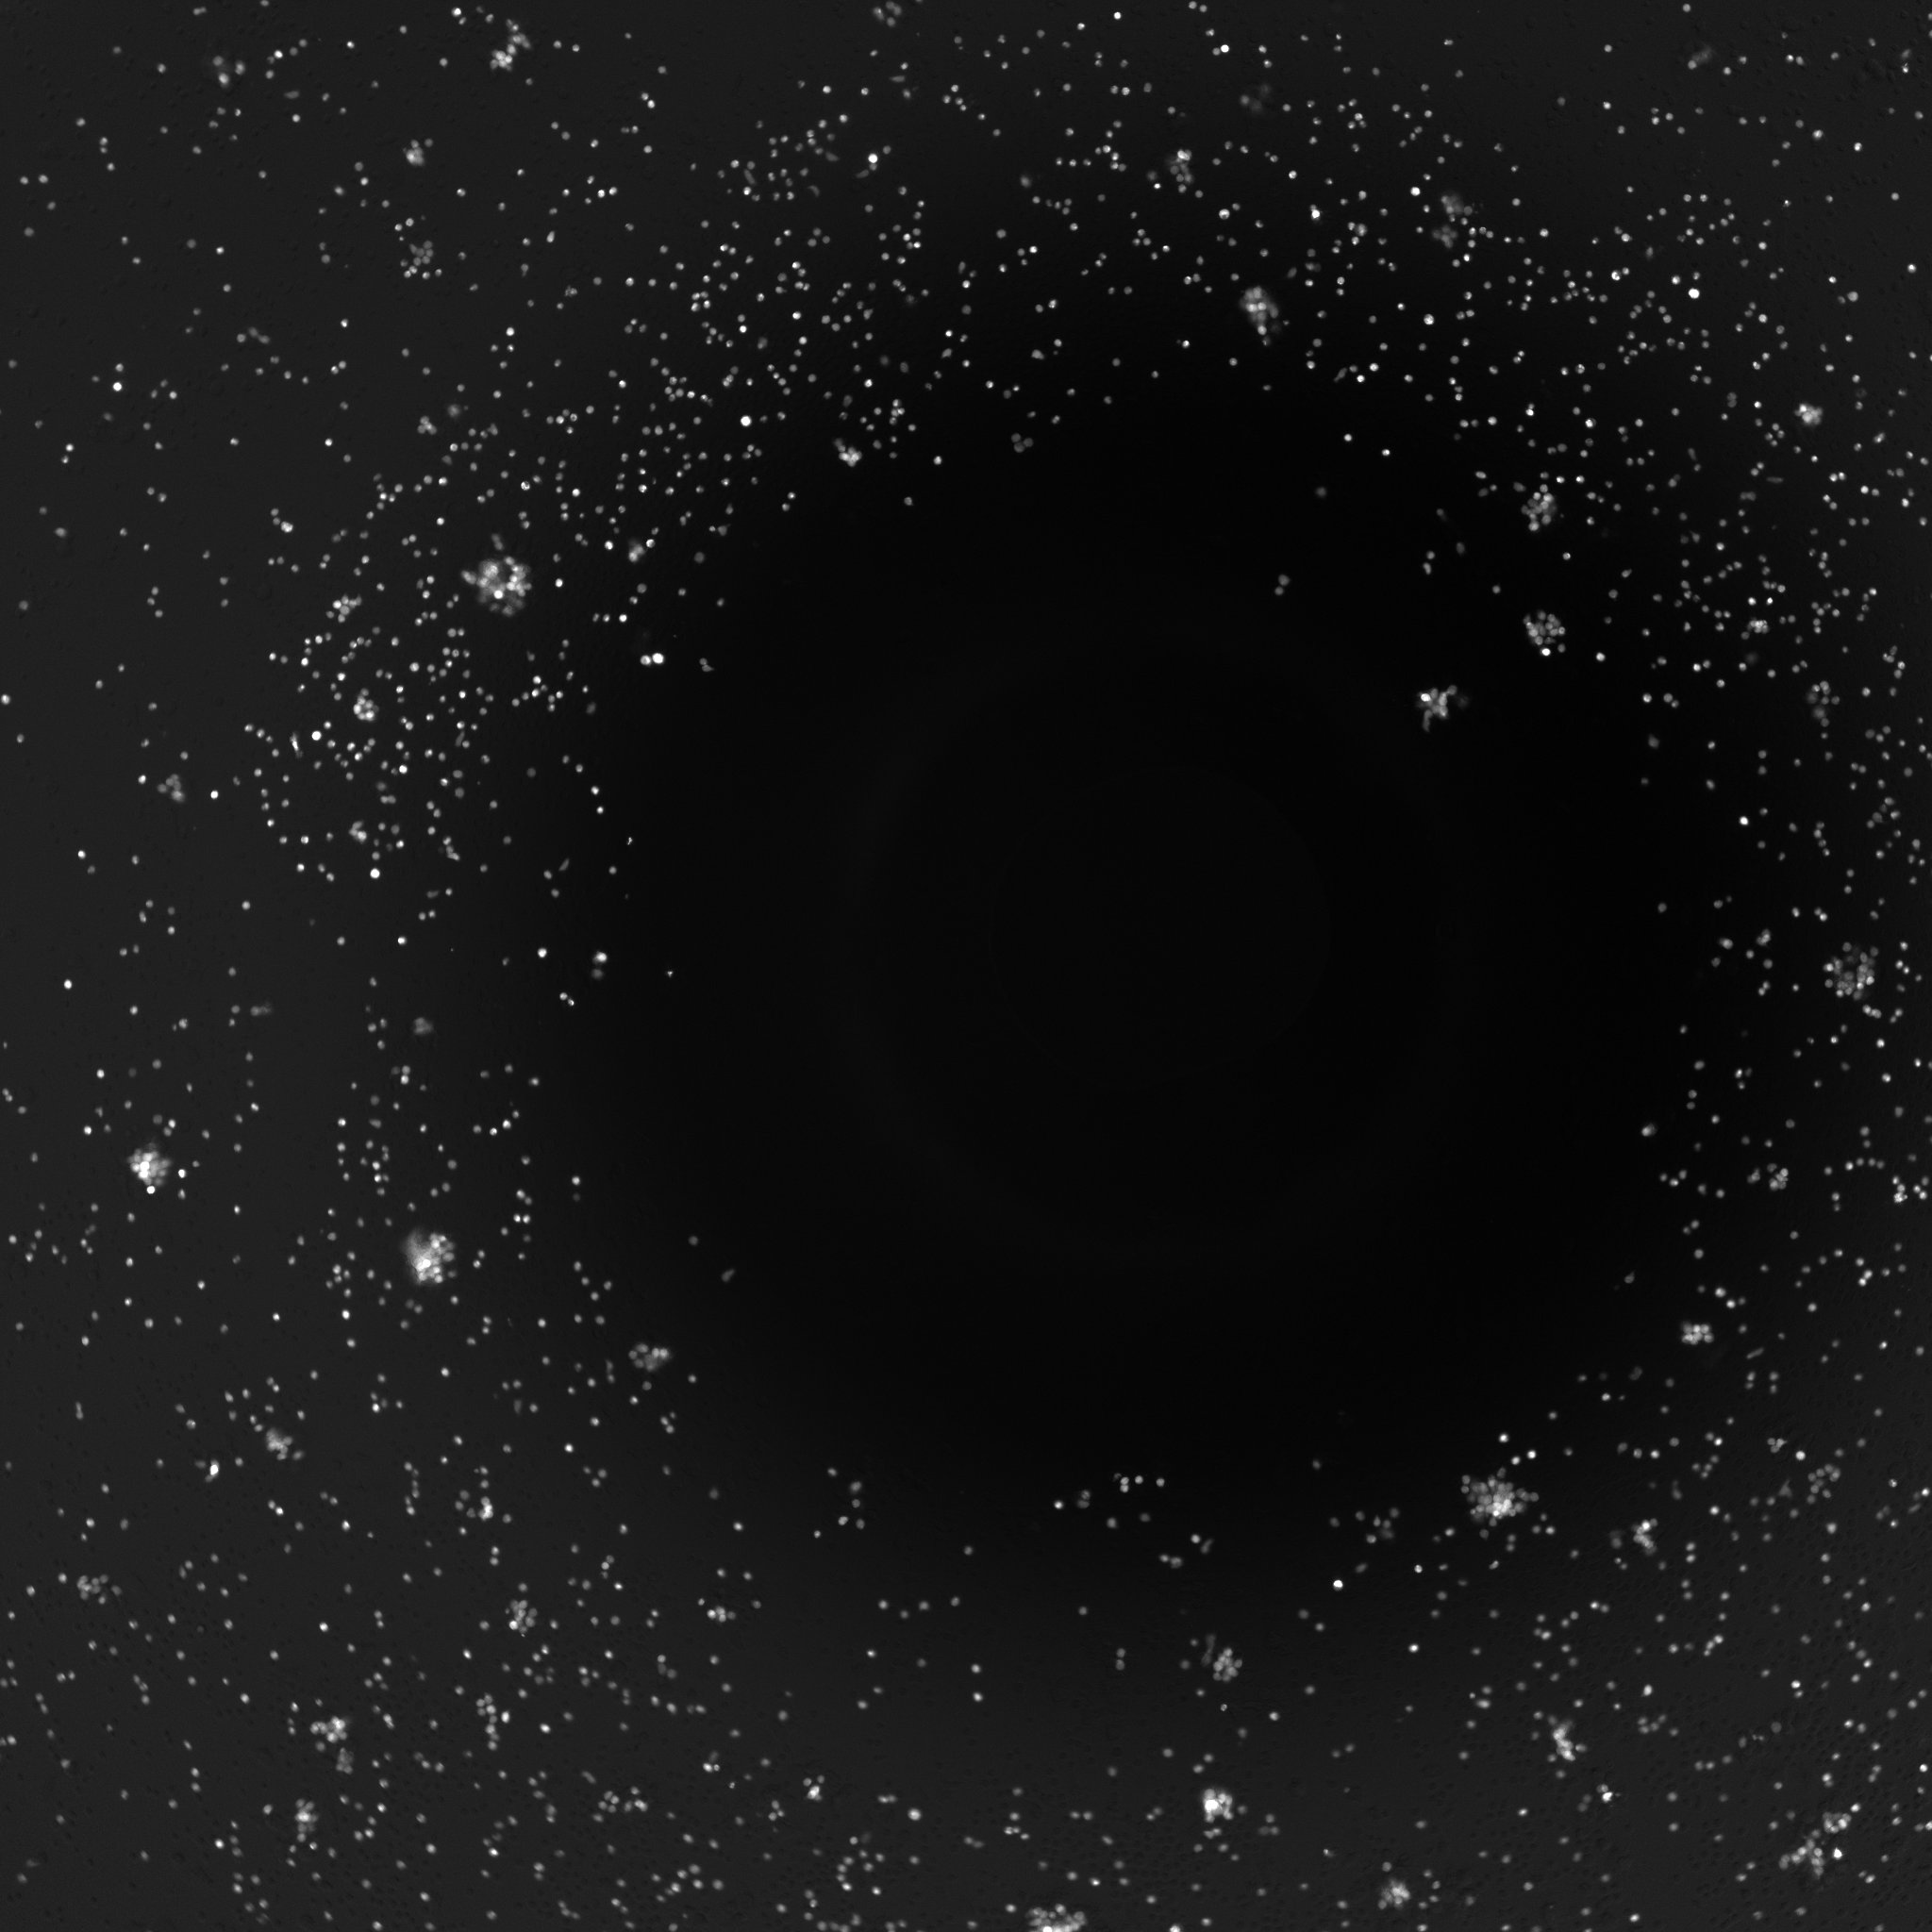
\includegraphics[width=\textwidth]{dissertation/figures/faulty_tcell.jpg}
        \caption{Green dye (T-cells) view}
        \label{subfig:tcell}
    \end{subfigure}
    \begin{subfigure}[h!]{0.3\textwidth}
        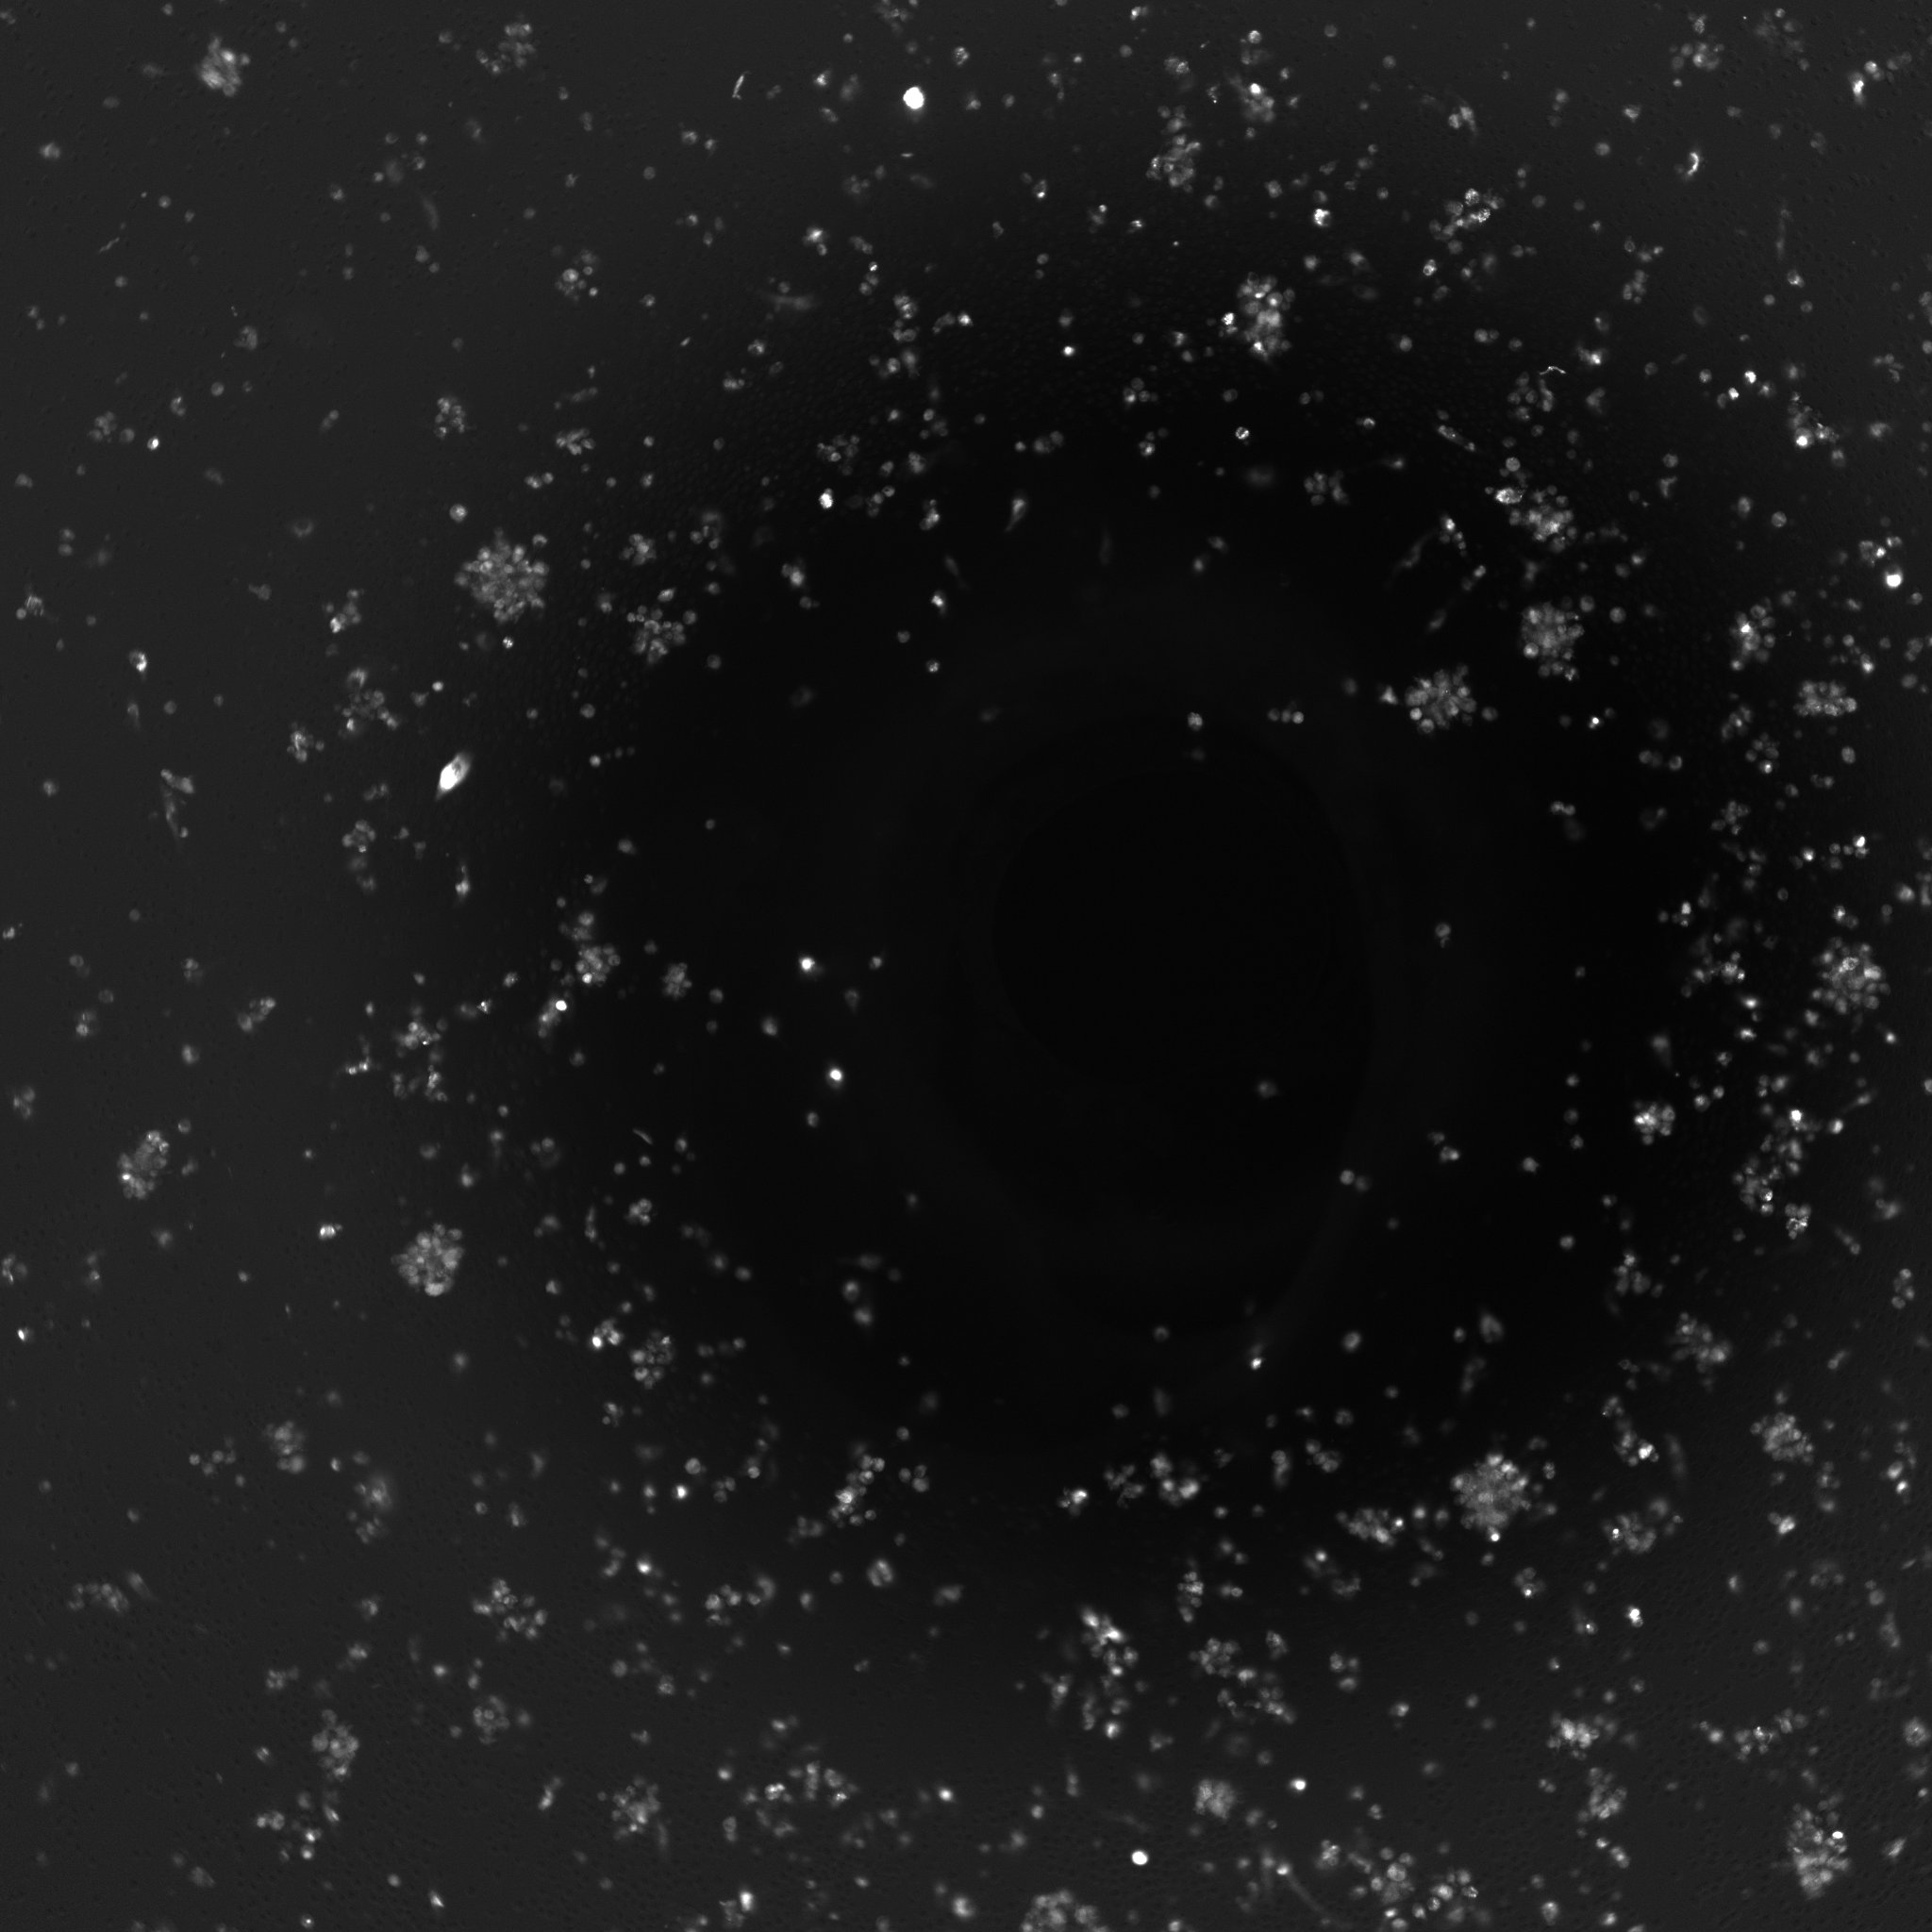
\includegraphics[width=\textwidth]{dissertation/figures/faulty_dcell.jpg}
        \caption{Red dye (DCs) view}
        \label{subfig:dc}
    \end{subfigure}
    \caption{Different views of an image which contains ``Faulty" patches. \protect\subref{subfig:tcell}, \protect\subref{subfig:dc} have been brightness-adjusted for visualisation.}
    \label{fig:noisyimage}
\end{figure}

\bigskip
\subsubsection{Labelling}

\hfill\\
\hfill\\
Each plate came with an Excel sheet giving information about the plate's layout. Each well was assigned a letter and a name, and the Excel sheet contained information about the stimulation, drug compound ID number, and compound concentration used for each well. These Excel sheets were not automatically parsable as types of drugs or location in the sheet might vary from one to the next, hence labelling had to be hardcoded and handchecked.

\subsection{Combining images to qualify interaction} \label{subsec:combining}

To summarise the section above, we made sure that for each well representing an experimental condition, we obtained two images of interest: an image of T-cells, and its counterpart image of dendritic cells. While these were obtained separately with the help of fluorescent dyes, they were still captured from the same well in which they were placed together. Hence, for us to gain any understanding of cell interaction from these images, we needed to combine them one way or another.

We decided to combine each black-and-white T-cell and DC image in one RGB image. Computationally speaking, an RGB image is represented by a multi-dimensional array of three arrays. Each of these arrays corresponds to a colour channel: red, green, or blue. The dendritic cell images were obtained through fluorescent red dye screening, so the red channel of the image was set to this image. Similarly, the T-cell images were obtained through fluorescent green dye screening, so the green channel of the image was set to this image. The blue channel of the RGB image was left blank. The resulting RGB image thus allowed us to visualise T-cells in green, DCs in red, with close overlap between those cells will in orange hues. Figure \ref{fig:combined} illustrates a sample of combined sub-images after this operation was completed.

This combination allowed us to visualise areas of proximity in cells as well as areas of overlap. As such, this visualisation provides us a means of qualifying interaction between the different types of immune cells.

\begin{figure}[h]
    \centering
    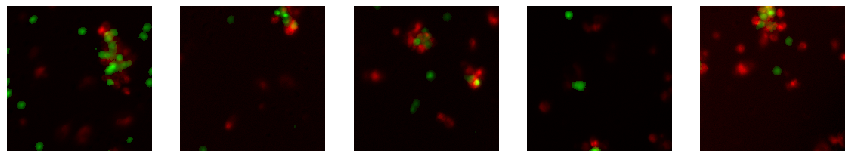
\includegraphics[width=\textwidth]{dissertation/figures/combined_cells.png}
    \caption{Random sample of five RGB images, where the red channel contains the dendritic cells and the green channel contains the T-cells.}
    \label{fig:combined}
\end{figure}

\section{Image segmentation}

Image segmentation refers to the process of separating out the parts of interest of an image into different `segments' or objects. In our context, applying image segmentation to our dataset had two purposes. The first was to use image segmentation as a method to separate the background from the cell objects for background correction. The second was to use it to obtain binary objects of the cells in order to compute numerical data about cells in the images.

\subsection{Background correction} \label{subsec:correction}

Although we have defined a method to perform some background noise reduction in images in Section \ref{subsec:preproc}, this method might not be able to catch all irregularities in the background. As such, we wanted to be cautious and explore some alternatives.

All the images in the original, uncombined dataset were black and white, with the details of interest (the cells) in bright white spots. However, as discussed in Section \ref{subsec:preproc}, the images could contain noise coming from grey details in the image that the naked eye cannot see immediately. Moreover, our noise removal methods might not be foolproof. There might be some noise remaining that could influence how a model learns. The best way for a model to learn about cells only is to only provide pixel values for cells, with a background sent to 0. Hence, we needed a method that will separate out the cell pixels from the background. We achieved this by obtaining a binary mask of the image, such that the white pixels of the binary image corresponded to the cells, and the dark pixels corresponded to the background. We tested two methods for doing this: K-means and thresholding, which will be described further in Section \ref{sec:implementation}.

Once a binary mask is obtained through these methods, we removed the background of the original image by multiplying it with the mask, a procedure known as \textit{masking}. If the binary mask is satisfactory, the output of this image should only contain the cells, which will have kept their detail, while the background will have been blacked out.

\subsection{Quantifying interaction}

The process used in \autoref{subsec:combining} describes a way of visually qualifying interaction between immune cells from combined images. However, we are also interested in quantifying interaction and obtaining a numeric value for the interaction between the T-cells and the dendritic cells.

We can use the same method as described in subsection \ref{subsec:correction} to obtain the mask of the cell objects in each image before combination. This pair of masks can be used for further calculations. A common metric for evaluating image segmentation quality is Intersection-over-Union (IoU), also known as the Jaccard index \citep{rahman_optimizing_2016, rezatofighi_generalized_2019, beers_deep_2019}. This metric is normally used to evaluate how successful the segmentation of an object in an image is by comparing the segmented object to its ground truth value. It is computed from binary objects as shown in \autoref{equation:iou}

\begin{equation}
    IoU(X,Y) = \frac{X \& Y}{X | Y}
    \label{equation:iou}
\end{equation}

In this case, we can use the IoU as a metric for area of overlap between two separate cell objects: the T-cell objects and the dendritic cell objects obtained from the same sub-image. We can use the concept of overlap to quantify the level of interaction between cells. These overlap numbers will be used as label input to a deep regression model. Each pair of images which will be combined and will be associated with an overlap value. The aim will be to evaluate whether we can train a model to predict a numeric value of interaction from an image.

\begin{figure}
    \centering
    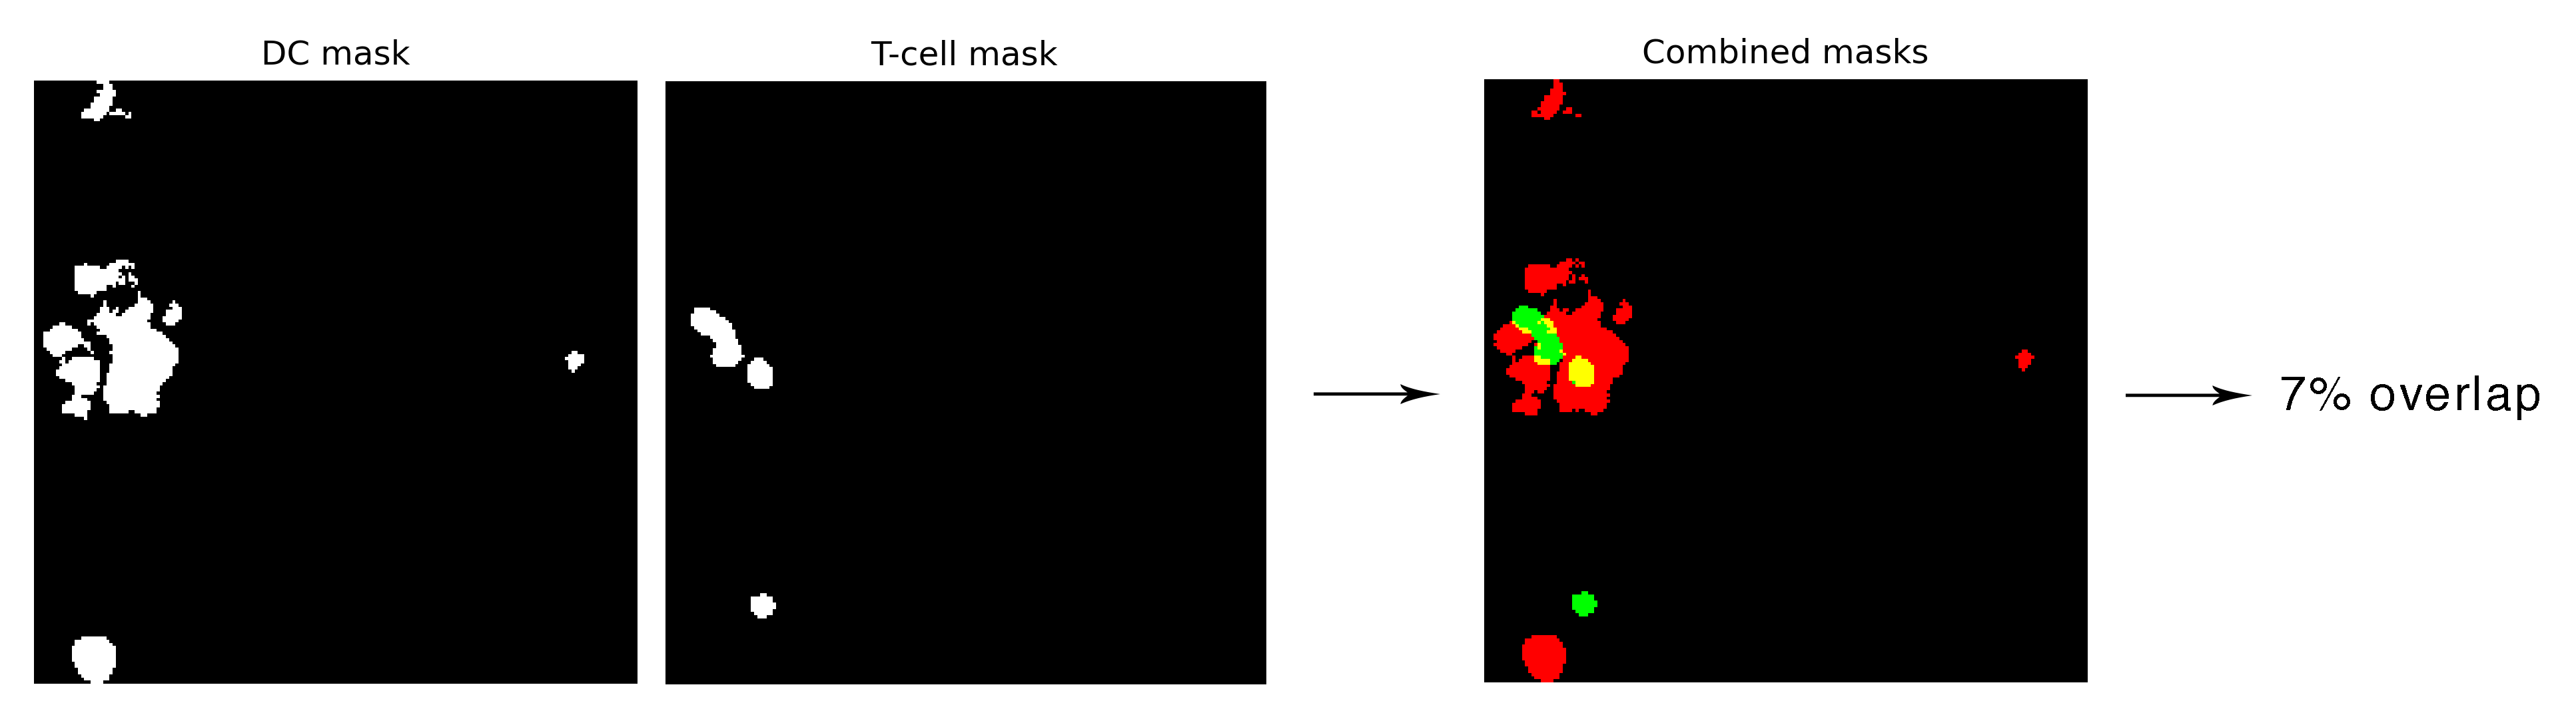
\includegraphics[width=0.8\textwidth]{dissertation/figures/mask_overlap_operation.png}
    \caption{Example of visual and numerical overlap between two sets of immune cells}
    \label{fig:mask_overlap}
\end{figure}

\section{Deep learning models}

The following two sections highlight what kind of deep learning models we used and their specific purposes of in the context of our research. Their general structure is highlighted in Figure \ref{fig:connected_models}.

\begin{figure}[h]
    \centering
    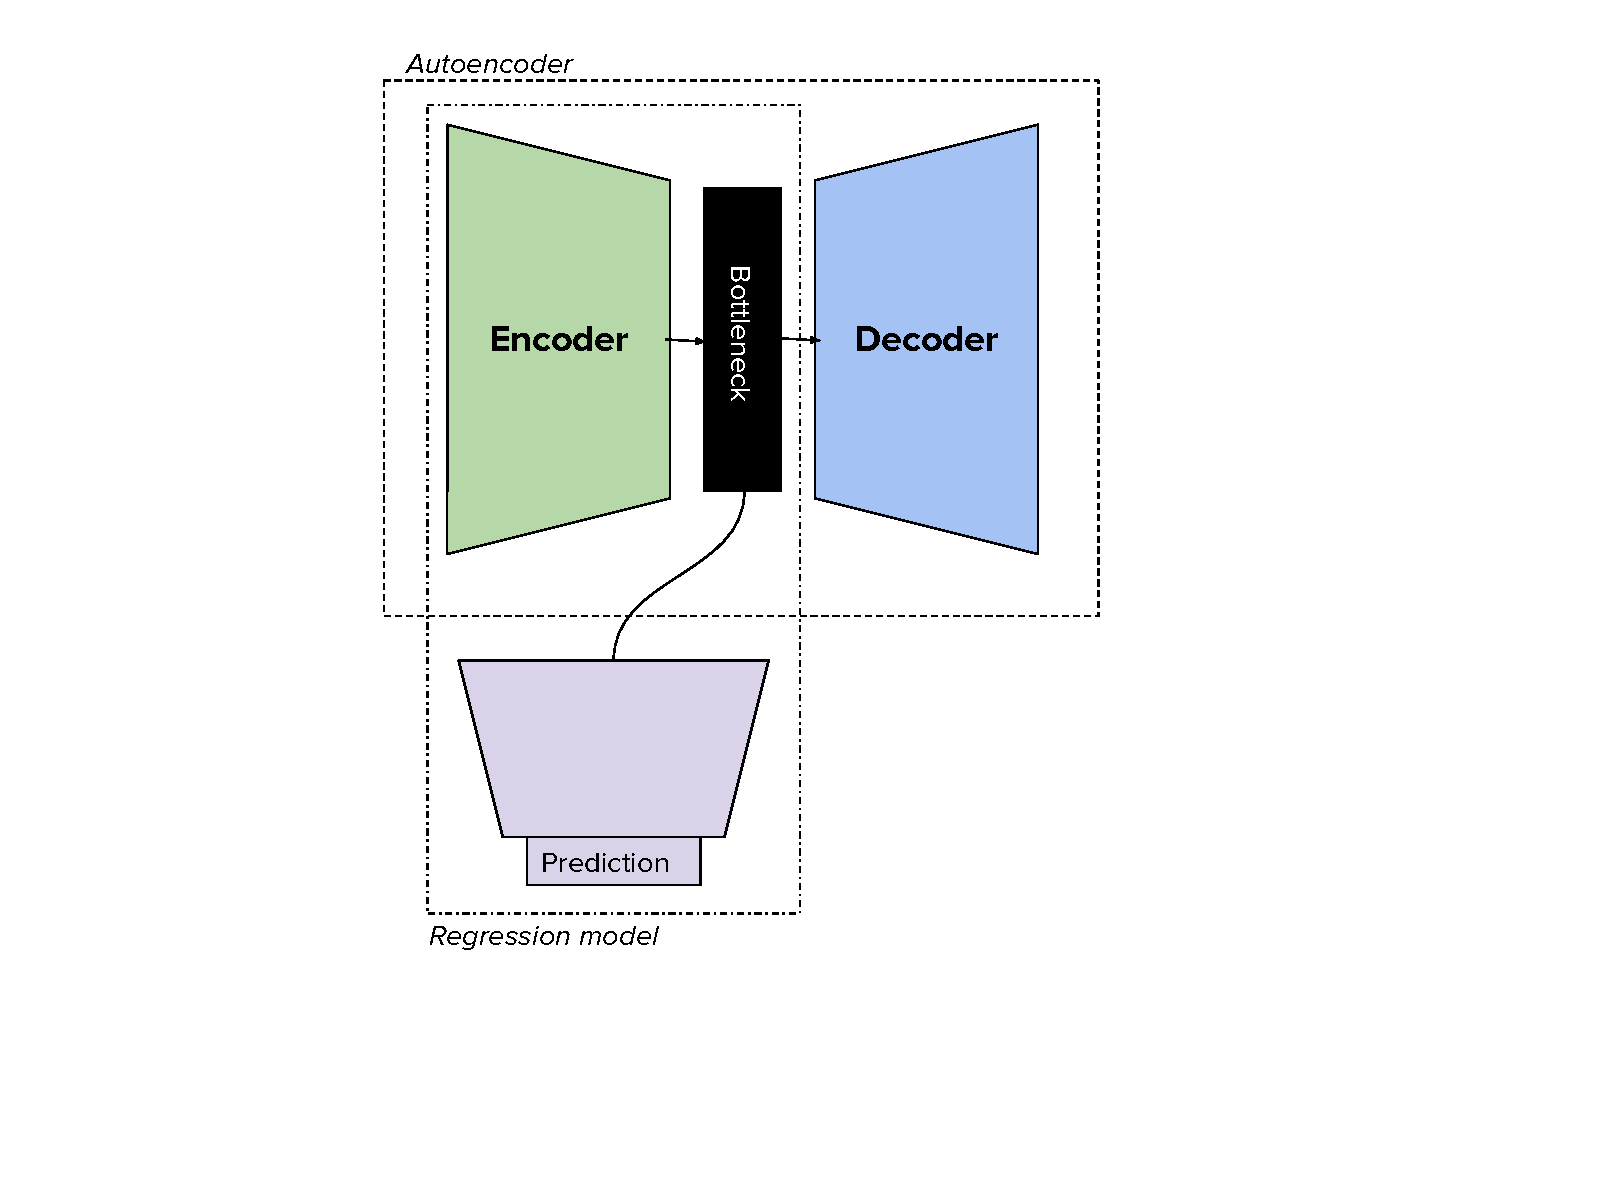
\includegraphics[width=.5\textwidth]{dissertation/figures/autoencoder_regression_connection.pdf}
    \caption{Schematic diagram of the models to be implemented. The encoder layers will transform the input into a smaller coded representation, from which the decoder layers will create a reconstructed version of the image. The encoder layers will then be connected to a regression model, from which we hope to make predictions on how much interaction is perceived in an image.}
    \label{fig:connected_models}
\end{figure}

\subsection{Autoencoder for visualising high dimensional data}

As described in Section \ref{sec:deepl_bg}, autoencoders are a particular type of neural network built with symmetrical layers around a bottleneck. The aim of an autoencoder is to map an input to itself as close as possible, while reducing its dimensions.

Different types of autoencoders exist. As our input consists of images, we set ourselves to implement a convolutional autoencoder. The hope was that if an image is reduced to a certain number of dimensions through convolutional neural networks, and another convolutional neural network is able to reconstruct the original image very closely just based on that compressed representation, then that smaller code representing an image is a good enough representation of the original input that can be fed into other models or algorithms.

The first aim for our autoencoder was to reduce the dimensions of our image input, as the size of the data points made it slow for data visualisation techniques to process. Furthermore, we hoped that the most important and distinguishing features of an image would come through the neural network layers and be collated in the bottleneck layer of the model.

High dimensionality visualisation techniques such as t-sne and UMAP can help visualise if there is an inherent structure to the data. We wanted to use this as a tool for analysis of immune cells interaction. We decided to use UMAP as our visualisation tool as both techniques yielded similar structures, but UMAP has been shown to outperform t-SNE time-wise. This also allowed us to experiment with UMAP's different parameters more easily, and to observe different structures of clusters in the data.

We wanted to be able to qualify interaction only from an image, without our model being supervised with labels about the image's experimental condition. This could be evaluated from a UMAP projection and whether or not clusters were formed around the same experimental conditions. If such successful groupings were found, it would allow us to show that different experimental conditions yield structurally similar cell interactions.

\subsection{Regression model for quantifying interaction in unseen images}

We also developed a deep regression model. Our regression task was to predict overlap values on unseen images. We used our autoencoder as a building block for a deep regression model. Again, we hoped that the autoencoder would successfully extract the most important features from the images through convolution operations and this would be a good starting block.

We used the encoder block of the model and extended it in a regression structure with fully connected layers. This regression model took images and associated overlap values as input for training. We could then assess whether or not the model successfully predicted interaction values from an image of T-cells and dendritic cells.
